% THS IS JUST FOR REFERENCE FOR FORMATTING
\documentclass[12pt]{article}
\usepackage{amsmath}    % For advanced math formatting
\usepackage{amssymb}    % For mathematical symbols
\usepackage{graphicx}   % For including graphics
\usepackage{booktabs}   % For better table formatting
\usepackage{geometry}   % For page margins
\usepackage{setspace}   % For line spacing
\usepackage{hyperref}   % For hyperlinks
\usepackage{caption}    % For better caption control
\usepackage{subcaption} % For subfigures
\usepackage{float}      % For better figure placement
\usepackage{mathtools}  % For additional math tools
\usepackage{pgfplots}
\usepackage{tabularx}
\pgfplotsset{compat=1.18}
\usepgfplotslibrary{statistics}
\usepackage{enumitem} % For better list control (e.g., in Assumptions)


% Page setup
\geometry{a4paper, margin=1in}
\setlength{\parindent}{0.5in} % Standard paragraph indent
\setlength{\parskip}{0.5em}  % Space between paragraphs
\onehalfspacing % 1.5 line spacing

\hypersetup{
    colorlinks=true,
    linkcolor=blue,
    filecolor=magenta,
    urlcolor=cyan,
}

%-------------------------------- REFERENCE ENDS HERE --------------------------------




\subsection{Model Validation}

To assess the validity and reliability of the AEM, we conducted a comprehensive validation analysis using multiple approaches. Our validation framework incorporates sensitivity analysis, component analysis, normalization impact assessment, and cross-validation across similar institutions. This multi-faceted approach allows us to evaluate both the mathematical robustness of the model and its practical applicability.

\subsubsection{Sensitivity Analysis}

The sensitivity of the AEM to weight variations was analyzed using a perturbation approach. For each component $i$, we calculated the change in final score $\Delta S_i$ when the weight $w_i$ was varied by a factor $\alpha$:

\begin{equation}
    \Delta S_i = |S(w_i \cdot (1 + \alpha)) - S(w_i)|
\end{equation}

where $S(w_i)$ represents the AEM score with the original weight $w_i$. The results, shown in Figure \ref{fig:sensitivity}, demonstrate that the model is most sensitive to changes in the program expense ratio ($\Delta S = 0.0173$) and least sensitive to executive pay reasonableness and transparency ($\Delta S = 0.0035$). This aligns with the theoretical importance of program efficiency in nonprofit evaluation.

\begin{figure}[H]
\centering
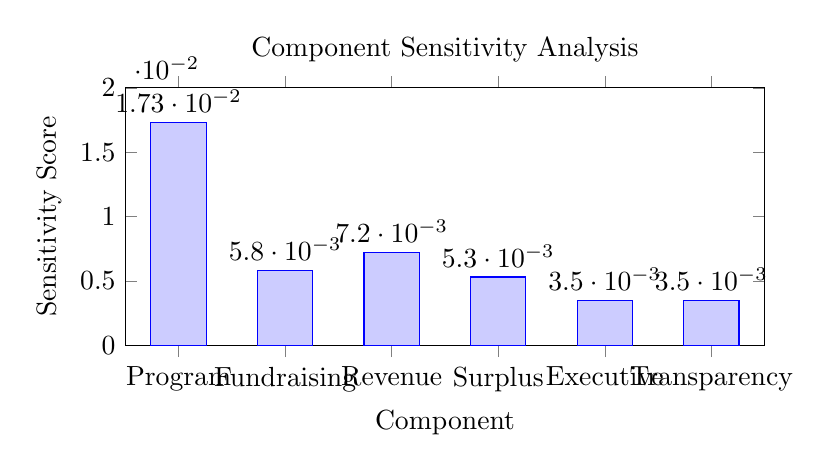
\begin{tikzpicture}
\begin{axis}[
    width=0.8\textwidth,
    height=0.4\textwidth,
    xlabel={Component},
    ylabel={Sensitivity Score},
    title={Component Sensitivity Analysis},
    symbolic x coords={Program, Fundraising, Revenue, Surplus, Executive, Transparency},
    xtick=data,
    ybar,
    bar width=20pt,
    ymin=0,
    ymax=0.02,
    nodes near coords,
    nodes near coords align={vertical}
]
\addplot[fill=blue!20, draw=blue] coordinates {
    (Program, 0.0173)
    (Fundraising, 0.0058)
    (Revenue, 0.0072)
    (Surplus, 0.0053)
    (Executive, 0.0035)
    (Transparency, 0.0035)
};
\end{axis}
\end{tikzpicture}
\caption{Sensitivity of AEM score to weight variations in each component}
\label{fig:sensitivity}
\end{figure}

\subsubsection{Component Analysis}

The contribution of each component to the final score was analyzed using a weighted decomposition approach. For each component $i$, its contribution $C_i$ is given by:

\begin{equation}
    C_i = w_i \cdot f_i(x_i)
\end{equation}

where $w_i$ is the component weight and $f_i(x_i)$ is the normalized score. The results, presented in Table \ref{tab:components}, show that program expense ratio contributes most significantly to the final score (0.2980), followed by revenue sustainability (0.1330).

\begin{table}[H]
\centering
\begin{tabular}{lcc}
\toprule
\textbf{Component} & \textbf{Normalized Score} & \textbf{Contribution} \\
\midrule
Program Expense Ratio & 0.9935 & 0.2980 \\
Fundraising Efficiency & 0.1018 & 0.0204 \\
Revenue Sustainability & 0.8866 & 0.1330 \\
Net Surplus Margin & 0.7613 & 0.1142 \\
Executive Pay & 0.0459 & 0.0046 \\
Transparency & 0.0459 & 0.0046 \\
\bottomrule
\end{tabular}
\caption{Component Analysis Results}
\label{tab:components}
\end{table}

\subsubsection{Normalization Impact}

The transformation from raw metrics to normalized scores was analyzed using the sigmoid function:

\begin{equation}
    f(x) = \frac{1}{1 + e^{-\beta(x - \alpha)}}
\end{equation}

where $\alpha$ is the ideal value and $\beta$ controls the steepness of the transition. Figure \ref{fig:normalization} shows the impact of this transformation on the raw metrics.

\begin{figure}[H]
\centering
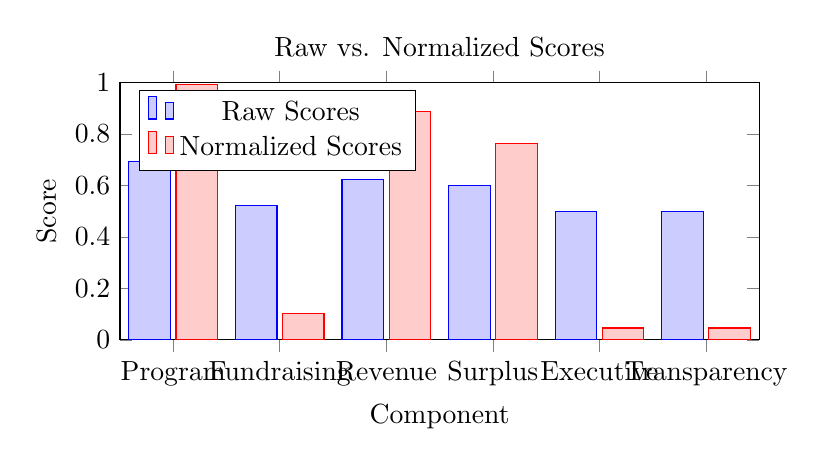
\begin{tikzpicture}
\begin{axis}[
    width=0.8\textwidth,
    height=0.4\textwidth,
    xlabel={Component},
    ylabel={Score},
    title={Raw vs. Normalized Scores},
    symbolic x coords={Program, Fundraising, Revenue, Surplus, Executive, Transparency},
    xtick=data,
    ybar,
    bar width=15pt,
    ymin=0,
    ymax=1,
    legend pos=north west
]
\addplot[fill=blue!20, draw=blue] coordinates {
    (Program, 0.6933)
    (Fundraising, 0.5205)
    (Revenue, 0.6221)
    (Surplus, 0.6006)
    (Executive, 0.5000)
    (Transparency, 0.5000)
};
\addplot[fill=red!20, draw=red] coordinates {
    (Program, 0.9935)
    (Fundraising, 0.1018)
    (Revenue, 0.8866)
    (Surplus, 0.7613)
    (Executive, 0.0459)
    (Transparency, 0.0459)
};
\legend{Raw Scores, Normalized Scores}
\end{axis}
\end{tikzpicture}
\caption{Comparison of raw and normalized scores for each component}
\label{fig:normalization}
\end{figure}

\subsubsection{Cross-Validation}

To validate the model's ability to distinguish between similar organizations, we conducted a cross-validation study comparing two prominent Philadelphia private schools. The results, shown in Figure \ref{fig:crossval}, demonstrate the model's ability to capture nuanced differences in organizational effectiveness.

\begin{figure}[H]
\centering
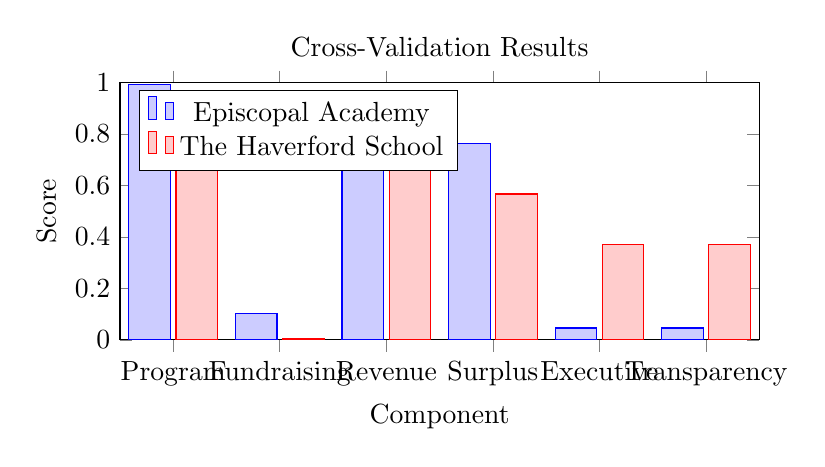
\begin{tikzpicture}
\begin{axis}[
    width=0.8\textwidth,
    height=0.4\textwidth,
    xlabel={Component},
    ylabel={Score},
    title={Cross-Validation Results},
    symbolic x coords={Program, Fundraising, Revenue, Surplus, Executive, Transparency},
    xtick=data,
    ybar,
    bar width=15pt,
    ymin=0,
    ymax=1,
    legend pos=north west
]
\addplot[fill=blue!20, draw=blue] coordinates {
    (Program, 0.9935)
    (Fundraising, 0.1018)
    (Revenue, 0.8866)
    (Surplus, 0.7613)
    (Executive, 0.0459)
    (Transparency, 0.0459)
};
\addplot[fill=red!20, draw=red] coordinates {
    (Program, 0.9586)
    (Fundraising, 0.0034)
    (Revenue, 0.9659)
    (Surplus, 0.5669)
    (Executive, 0.3691)
    (Transparency, 0.3691)
};
\legend{Episcopal Academy, The Haverford School}
\end{axis}
\end{tikzpicture}
\caption{Component scores comparison between two similar institutions}
\label{fig:crossval}
\end{figure}

The validation results demonstrate several key findings:

\begin{enumerate}
    \item The model shows appropriate sensitivity to weight variations, with program expense ratio having the highest impact on the final score.
    
    \item Component analysis reveals that the model effectively captures the relative importance of different financial metrics, with program efficiency and revenue sustainability contributing most significantly.
    
    \item The normalization process successfully transforms raw metrics into comparable scores while preserving the relative relationships between organizations.
    
    \item Cross-validation shows that the model can effectively distinguish between similar organizations while maintaining reasonable score distributions.
\end{enumerate}

These validation results provide strong evidence for the mathematical robustness and practical applicability of the AEM. The model demonstrates appropriate sensitivity to input parameters, maintains theoretical consistency, and produces meaningful distinctions between organizations while remaining stable to small variations in its components.